\chapter{Точностные расчеты ОЭП. Методы повышения качества ОЭП}
\section{Точностные критерии качества ОЭП}

Одним из важнейших критериев качества ОЭП является точность, определяемая потерями информации, которые приводят к погрешностям средств измерений и контроля.

Обеспечение заданной точности измерения --- одна из главных задач, встающих перед разработчиком уже на первых этапах проектирования ОЭП. Решение ее достигается путем расчета основных метрологических параметров ОЭП и сопоставления их с требованиями технического задания (ТЗ). Результаты точностных расчетов помогают определить требования к отдельным узлам прибора, допуски на погрешности их изготовления и сборки, допуски на параметры и характеристики элементов ОЭП и многие другие. От того, насколько правильно будут решены вопросы выявления и учета погрешностей, назначения допусков, зависят показатели качества информации, передаваемой ОЭП, его технологичность и надежность.

В обобщенном случае схему функционирования ОЭП можно представить в виде, показанном на рис.~\ref{pic:10scheme}, где $ x_{0i} $, $ x_i $, $ y_i $~-- $ i $-е информативные параметры объекта, входного и выходного сигналов соответственно; $ q_i $~-- $ i $-й схемный (конструктивный) параметр прибора; $ f_i $~-- функция, связывающая $ x_i $ и $ y_i $ ; $ \text{ФУ}_1 $, $ \text{ФУ}_2,\ldots,\,\text{ФУ}_n $~-- функциональные устройства прибора; $ q'_j $~-- влияющие факторы, $ f'_i $~-- функция, связывающая $ y_i $ с $ x_{0i} $.

Процесс функционирования ОЭП, как, впрочем, и каждого прибора, сопровождается погрешностями (потерей информации), которые характеризуют точность результата функционирования, т.е. точность измерения, управления или обнаружения, осуществляемого прибором.

\begin{figure}[h!]
%	\caption{ Схема функционирования оптико-электронного прибора:\\ 1~-- объект наблюдения, 2~-- оптико-электронный прибор, \\3~-- оператор (устройство управления, регулирования) }
	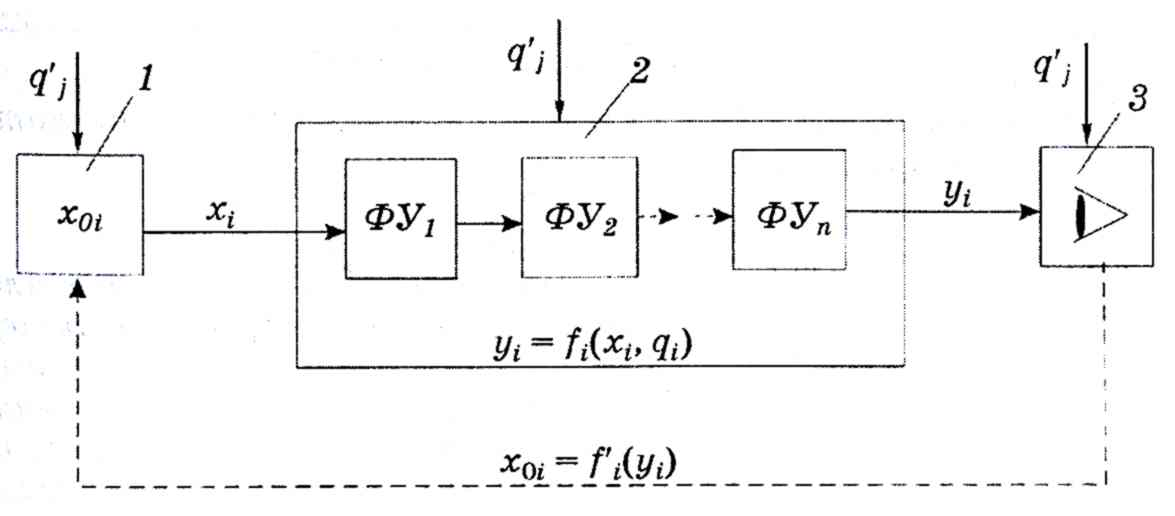
\includegraphics[width=0.9\textwidth]{10scheme.png}
	\label{pic:10scheme}
\end{figure}

В общем случае погрешность результата функционирования прибора обусловлена потерей информации, возникающей до преобразования входного сигнала в приборе, непосредственно в процессе преобразования и при регистрации и обработке результатов. 

Погрешности из-за потери информации до преобразования ее в приборе, а также при регистрации и обработке, называют обычно методическими погрешностями.

Погрешности, обусловленные потерей информации в оптических, механических, электронных и других ФУ прибора, осуществляющих преобразование информативного параметра входного сигнала в информативный параметр выходного сигнала, называют инструментальными (аппаратурными, приборными).

\section{Методические погрешности}

Методические погрешности обусловлены ошибочностью или недостаточностью разработки принятой теории метода функционирования прибора в целом, допущениями в отношении объекта, сигнала или канала прохождения сигнала, неправильной ориентировкой прибора относительно объекта, дискретностью представления информации и т.п.

Методические погрешности, связанные с допущениями, особенно характерны для измерительных приборов, принцип действия которых основан на косвенных методах измерения.

Рассмотрим два примера.

\begin{flushleft}
\textbf{Пример 1}
\end{flushleft}

В функции, заложенной в основу работы импульсных светодальномеров (рис.~\ref{pic:10dalnomer}), $ D = ct/2n $ (где $ D $~-- дистанция до объекта; $ c $~-- скорость света в вакууме; $ t $~-- время прохождения излучения до объекта и обратно (измеряемый параметр), $ n $~-- показатель преломления среды), предполагается, что показатель преломления среды на трассе измерения постоянен и равен некоторому конкретному значению.

\begin{figure}[h!]
	\caption{ Схема работы светодальномера }
	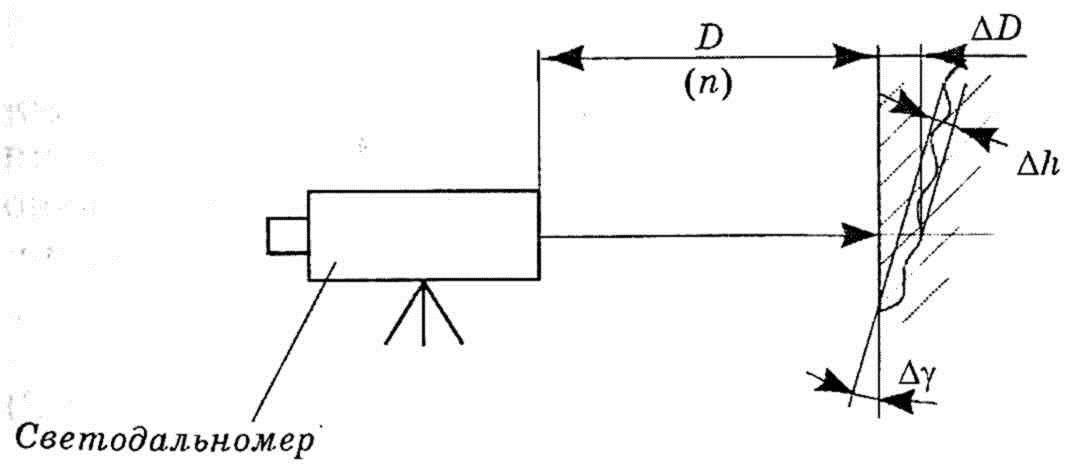
\includegraphics[width=1\textwidth]{10dalnomer.png}
	\label{pic:10dalnomer}
\end{figure}

При реальных измерениях значение этого параметра известно только приблизительно, к тому же он изменяется на различных участках трассы, что приводит к методической погрешности измерения дистанции:
\[ \Delta D_{\Delta n} = \dfrac{c\,t}{2n^2}\Delta n = - \dfrac{D}{n}\Delta n \]
К методическим погрешностям измерения дистанции будут относиться также погрешности, обусловленные наклоном $ \Delta\gamma $ и неровностями (шероховатостью) $ \Delta h $ формы поверхности объекта.

\begin{flushleft}
\textbf{Пример 2}
\end{flushleft}

В том случае, когда в основу функционирования прибора, например нивелира~1 (рис.~\ref{pic:10nivelir}), положено допущение о прямолинейном распространении пучка лучей от прибора до объекта (рейки~2), к методической погрешности следует отнести погрешность $ \Delta H $ измерения высоты из-за рефракции воздушных слоев, приводящих к искривлению линии визирования (например, на 100~м $ \Delta H $ может достигать 1-2~мм).

\begin{figure}[h!]
	\caption{ Схема работы нивелира }
	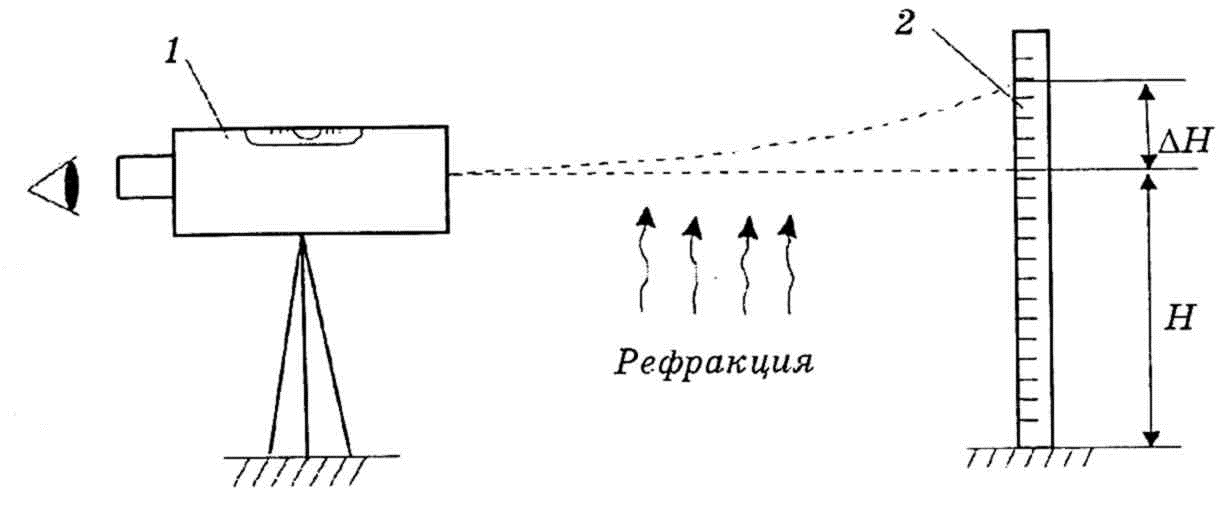
\includegraphics[width=1\textwidth]{10nivelir.png}
	\label{pic:10nivelir}
\end{figure}

Отличительной особенностью методических погрешностей является то, что они обязательно связаны с результатом функционирования прибора (измерения, управления, обнаружения объекта) и определяются путем создания математической модели или имитационным моделированием метода и объекта, а не могут быть найдены только исследованием самого прибора.

\section{Инструментальные погрешности}

Инструментальные погрешности подразделяются на теоретические, технологические и эксплуатационные.

Теоретические погрешности. Обусловлены тремя видами допущений:
\begin{itemize}
\item структурными --- допущениями в законе функционирования прибора, в функции $ f_i $, связывающей информативные параметры входного $ x_i $, и выходного $ y_i $ сигналов (рис.~\ref{pic:10scheme});
\item параметрическими --- допущениями в значениях конструктивных параметров $ q_i $;
\item конструктивными --- допущениями в конструкциях высших кинематических пар.
\end{itemize}

Теоретические погрешности первого вида (структурные, схемные) возникают при замене точной функции преобразования сигнала приближенной зависимостью. Чаще всего это происходит, когда вместо нелинейной функции пользуются ее линейным приближением.

Теоретические погрешности второго вида (параметрические) обусловлены округлениями конструктивных параметров до значений, нормируемых стандартами, и округлениями иррациональных параметров.

Оптикам хорошо известно правило, согласно которому необходимо при расчетах радиусов кривизны поверхностей оптических деталей округлять полученные значения до ближайших радиусов по ГОСТ~1807-75. Естественно, что в результате этого несколько изменяются исходные (или искомые) характеристики оптических систем.

Теоретические погрешности третьего вида (конструктивные) обычно возникают при конструировании высших кинематических пар кулачковых и рычажных механизмов.

\section{Технологические погрешности}

Технологические погрешности возникают в процессе изготовления и сборки элементов ОЭП и могут быть следующими:
\begin{itemize}
\item отклонения от расчетных значений характеристик материалов деталей (например, показателя преломления и средней дисперсии стекла, модуля упругости, коэффициента линейного расширения);
\item погрешности размеров и форм деталей, возникающие при их изготовлении (например, погрешности радиусов кривизны и формы рабочих поверхностей линз, клиновидности призм, погрешности деления шкал, погрешности форм поверхностей направляющих);
\item погрешности расположения и деформации деталей, возникающие при их сборке (например, децентрировки и деформации линз, перекосы шкал, погрешности значений воздушных промежутков).
\end{itemize}

К технологическим погрешностям часто относят погрешности параметров и характеристик покупных (стандартизованных, унифицированных) элементов и блоков (подшипников, приемников, шаговых двигателей, датчиков, АЦП), так как их погрешности обусловлены комплексными дефектами изготовления.

Однако если значения этих погрешностей известны (паспортизованы) и могут быть приписаны конкретным значениям информативного параметра выходного сигнала у прибора, то их относят к теоретическим погрешностям.

Технологические погрешности --- это один из самых многочисленных и наиболее сильно влияющих на точность функционирования и качество изображения ОЭП источников погрешностей.

\section{Эксплуатационные погрешности}
Эксплуатационные погрешности возникают из-за воздействия на ОЭП внешних и внутренних влияющих факторов: нагрузок, вибраций, сил трения, температуры, давления, влажности, радиационного излучения, электромагнитных полей, нестабильности источников питания.

Влияние этих факторов приводит: к изменению характеристик материалов (например, показателя преломления стекла при изменении температуры); изменению размеров, формы и положения деталей (например, радиусов и формы кривизны поверхностей, диаметров линз, длин плеч рычагов, значений воздушных промежутков между оптическими деталями, положения осей в подшипниках); изменению характеристик и параметров покупных изделий (например, чувствительности приемников, излучательной способности источников излучения).

Особенностью инструментальных погрешностей является то, что они могут быть измерены (исследованы) и занесены в паспорт прибора (устройства).

Погрешности можно классифицировать различным образом:
\begin{itemize}
\item по размерности --- абсолютные и относительные;
\item по характеру связи с измеряемой величиной --- аддитивные, мультипликативные;
\item по закономерности появления --- систематические и случайные;
\item по причинам появления --- методические и инструментальные;
\item по условиям появления --- статические и динамические.
\end{itemize}

\textit{Абсолютная погрешность} измерений, выражаемая в единицах измеряемой величины, представляется разностью между измеренным и истинным (действительным) значениями измеряемой величины. 

\textit{Относительная погрешность}~--- отношение абсолютной погрешности к истинному (действительному) значению измеряемой величины и выражается в процентах или долях измеряемой величины.

\textit{Аддитивной погрешностью} называется погрешность, постоянная в каждой точке шкалы.

\textit{Мультипликативной погрешностью} называется погрешность, линейно возрастающая или убывающая с ростом измеряемой величины.

\textit{Случайная погрешность}~--– это составляющая погрешности измерения, изменяющаяся случайным образом при повторных измерениях одной и той же величины. 

\textit{Систематической погрешностью} называется составляющая погрешности измерения, остающаяся постоянной или закономерно меняющаяся при повторных измерениях одной и той же величины.

\textit{Статическая погрешность измерений}~--- погрешность результата измерений, свойственная условиям статического измерения, то есть при измерении постоянных величин после завершения переходных процессов в элементах приборов и преобразователей. 

\textit{Динамическая погрешность измерений} --- погрешность результата измерений, свойственная условиям динамического измерения. Динамическая погрешность появляется при измерении переменных величин и обусловлена инерционными свойствами средств измерений.

\section{Классификация погрешностей}

Рассмотрим классификацию погрешностей в зависимости от их причинно-следственной структуры и свойств. Структура погрешностей прибора (устройства) приведена на рис.~\ref{pic:10error}.

\begin{figure}[h!]
	\caption{ Причинно-следственная структура погрешностей прибора }
	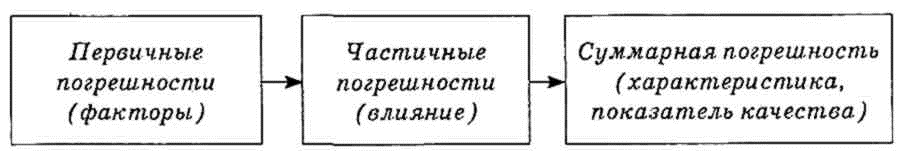
\includegraphics[width=0.8\textwidth]{10error.png}
	\label{pic:10error}
\end{figure}

Первичные погрешности и факторы представляют собой: 
\begin{itemize}
\item отклонения $ \Delta q $ от номинальных значений конструктивных параметров и характеристик деталей (размеров, формы, расположения, характеристик материалов) и сборочных единиц. Погрешности конструктивных параметров и характеристик сборочных единиц являются комплексными, обусловленными первичными погрешностями изготовления и сборки входящих в них деталей и элементов. Обычно в качестве комплексных первичных погрешностей принимают погрешности (стандартизированных) покупных изделий и погрешности унифицированных сборочных единиц, нормируемых комплексным показателем точности (например, погрешностью фокусного расстояния объектива и т.п.);
\item изменения $ \Delta q' $ влияющих факторов (освещенность, температура, внешний шум);
\item отклонение $ \Delta f $ от расчетного значения функции преобразования сигнала (например, отклонение от синусоидального или квадратичного);
\item отклонения $ \Delta x $ информативного параметра сигнала, поступающего на вход прибора, от его номинального значения  из-за методических допущений (например, в дальномере искажение формы импульса при его отражении от мишени и распространении в атмосфере).
\end{itemize}

Заметим, что первичные факторы   приводят к изменению конструктивных параметров и характеристик деталей и сборочных единиц, т.е. они оказывают влияние на точность прибора через  . При этом один первичный фактор (например, изменение температуры может приводить к изменению фокусного расстояния объектива за счет температурных деформаций линз и изменению расстояния между ними) может действовать на изменение как одного, так и нескольких конструктивных параметров и характеристик одновременно.

Каждая отдельная первичная погрешность и фактор влияют на точность прибора. Это влияние (т.е. единичное действие первичной погрешности или фактора на информативный параметр выходного сигнала, а стало быть, и на характеристику точности) называется частичной (частной) погрешностью (частичным влиянием) и обозначается $ \Delta y_{\Delta q},\,\Delta y_{\Delta q'},\,\Delta y_{\Delta f},\, \Delta y_{\Delta x} $.

Частичная погрешность (в общем случае) равна произведению первичной погрешности $ \Delta q $ на некоторую функцию $ A_q $:
\[ \Delta y_{\Delta q} = A_q\,\Delta q. \]

Эта функция, связывающая частичную погрешность с первичной погрешностью или фактором, может быть в общем виде как линейной, так и нелинейной и называется передаточной функцией (коэффициентом влияния) первичной погрешности (фактора).

Частичные погрешности, суммируясь, образуют суммарную погрешность прибора (устройства) $ \Delta y_\Sigma $ .

В общем случае можно считать, что суммарная погрешность (показатель качества) равна алгебраической сумме частичных погрешностей
\begin{equation}
\label{eq:10ysum}
\Delta y_\Sigma = \sum\limits_{i}^{n} \Delta y_{\Delta q_i},
\end{equation}
где $ n $ --- число частичных погрешностей.

Определяющий номенклатуру основных метрологических характеристик ГОСТ~8.009-84 <<Нормируемые метрологические характеристики средств измерения>> регламентирует разделение инструментальной погрешности на следующие составляющие:
\begin{enumerate}
\item погрешность, вызванная неидеальностью отдельных звеньев ОЭП, например наличием шумов, люфтов, дрейфов параметров, что приводит к отличию реальной функции преобразования~-- зависимости между выходным сигналом и входным (информативным параметром), характерной для нормальных (стандартных) условий функционирования ОЭП, от идеальной функции преобразования (статической характеристики). Эта составляющая называется основной погрешностью прибора;
\item  погрешность, обусловленная реакцией прибора на изменения внешних влияющих факторов и неинформативных параметров входного сигнала относительно их номинальных значений. Эта составляющая называется дополнительной погрешностью;
\item погрешность, возникающая как реакция прибора на скорость или частоту изменения входного сигнала. Она, как и основная погрешность, зависит от свойств отдельных звеньев прибора, например от их инерционности, но выделяется как отдельная составляющая и называется динамической погрешностью.
\end{enumerate}

Первые две составляющие образуют статическую погрешность.

На практике часто удобно из общей погрешности выделить следующие составляющие:
\begin{itemize}
\item Методическую. В основном методическая погрешность носит систематический характер, однако в общем случае она содержит и случайную составляющую, оцениваемую, например, дисперсией $ \sigma^2_\text{мет} $. Часто эту оценку можно учесть с достаточно высокой достоверностью;
\item Инструментальную. Ряд факторов, определяющих инструментальную погрешность, носит систематический характер, другие --- случайный, причем некоторые из последних выделяются в отдельную составляющую. Опыт, накопленный оптико-электронным приборостроением, позволяет с достаточной достоверностью рассчитывать и учитывать как систематическую, так и случайную составляющую (например, дисперсию $ \sigma^2_\text{и} $) инструментальной погрешности;
\item Динамическую, обусловленную инерционностью ОЭП и отдельных его звеньев. Случайная составляющая динамической погрешности может быть оценена дисперсией  $ \sigma^2_\text{дин} $.
\item Флуктуационную, к которой относят часть случайных составляющих инструментальных погрешностей, например возникающих вследствие шумов приемника излучения и электронных звеньев ОЭП, а также случайные составляющие, вызванные внешними помехами и шумами. Обозначим дисперсию флуктуационной погрешности через $ \sigma^2_\text{фл} $.
\end{itemize}

Очень важно правильно учесть характер взаимодействия отдельных составляющих суммарной погрешности прибора или измерения. 
Допустим, что систематическая составляющая инструментальной погрешности может быть устранена или учтена, а случайные составляющие общей погрешности некоррелированы между собой и складываются квадратически, т.е. дисперсия суммарной погрешности (характеризующая случайные составляющие)
\[ \sigma^2_\Sigma = \sigma^2_\text{м} + \sigma^2_\text{и} + \sigma^2_\text{дин} + \sigma^2_\text{фл} \]
где $ \sigma^2_\Sigma,\, \sigma^2_\text{м},\,\sigma^2_\text{и},\,\sigma^2_\text{дин},\,\sigma^2_\text{фл} $ --- дисперсии случайных составляющих общей (суммарной) погрешности и ее составляющих: методической, инструментальной, динамической и флуктуационной. Здесь динамическая и флуктуационная (обусловленная шумами и помехами внутреннего и внешнего происхождения) составляющие выделены из общей инструментальной погрешности).

В этом случае иногда на стадии предварительного проектирования ОЭП с учетом известного характера и знания ориентировочных величин $ \sigma^2_\text{м} $ и $ \sigma^2_\text{и} $ можно выделить совокупность $ \sigma^2_\text{дин} $ и $ \sigma^2_\text{фл} $, т.е. для допустимого значения $ \sigma^2_\Sigma $ принимать как допуск
\[ \sigma^2_\text{дин} + \sigma^2_\text{фл} = \sigma^2_\Sigma - (\sigma^2_\text{м} + \sigma^2_\text{и})  \]
и на первых этапах точностного расчета ОЭП определять составляющие $ \sigma^2_\text{дин} $ и $ \sigma^2_\text{фл} $.

При разработке новых ОЭП или при оценке точностных возможностей уже созданных ОЭП в условиях эксплуатации, существенно отличающихся от прежних, т.е. при априорной неопределенности отдельных составляющих погрешностей, целесообразно провести точностной расчет прибора в несколько этапов.

\section{Точностные расчеты ОЭП}

\begin{flushleft}
\textbf{Основные этапы точностных расчетов}
\end{flushleft}

Точностные расчеты ОЭП и их отдельных узлов можно разделить на две группы: проектные (точностный синтез) и проверочные (точностный анализ).

Расчеты, относящиеся к первой группе, проводят в начале проектирования прибора. Они позволяют оптимизировать принцип функционирования ОЭП, определить рациональную структуру ОЭП, а также установить некоторые исходные данные для назначения допусков на погрешности отдельных его узлов и элементов исходя из требований технического задания (ТЗ) к точности с учетом условий производства, эксплуатации, требований соответствующих ГОСТов, стоимости.

Задачи точностного анализа заключаются в определении количественных оценок точности (суммарной погрешности) проектируемого устройства при выбранных в процессе его проектирования принципе функционирования, схемах, конструктивных параметрах, допусках на элементы с учетом известных влияющих факторов.

Первым этапом точностного расчета для вновь разрабатываемого ОЭП может являться расчет потенциальной его точности, т.е. точности оптимальной системы, характеризующей идеализированную измерительную схему без учета структуры ОЭП, свойств его звеньев (методических, инструментальных, динамических и флуктуационных погрешностей, определяемых параметрами и характеристиками звеньев ОЭП) и часто обусловленной лишь свойствами принимаемого сигнала и внешних помех. Значение погрешности, определяющей потенциальную точность, характеризует предельно достижимое качество измерений, а также задает тот предел, к которому может стремиться разработчик прибора. Если значение этой погрешности превышает значение, установленное техническим заданием, то при активном методе работы ОЭП следует просмотреть возможность изменения параметров сигнала, посылаемого передающей оптической системой к приемной, а в более общем случае постараться уменьшить влияние внешних шумов и помех.
 
После выбора предварительной структурной схемы прибора и значений основных параметров его звеньев необходимо рассчитать динамические и флуктуационные погрешности. При этом, опираясь на опыт предшествующих разработок, иногда можно определить допустимое значение их суммы по формуле \eqref{eq:10ysum}. Прежде чем приступить к этому расчету, обычно следует выполнить энергетические расчеты отдельных звеньев прибора. Например, зная мощность поступающего на приемник излучения, можно определить структуру электронного канала и рассчитать значение его коэффициента усиления.

Расчет динамических и флуктуационных погрешностей позволяет выбрать оптимальную структуру прибора, его основные параметры, подобрать корректирующие звенья. Критерием оптимизации является минимум $ \sigma^2_\text{дин} $ и $ \sigma^2_\text{фл} $.

Следующим этапом точностного расчета, проведение которого необходимо после разработки реальной конструкции прибора, является расчет инструментальной погрешности, включающей динамические и флуктуационные погрешности реальных звеньев, а также погрешности, обусловленные неточностью изготовления и сборки этих звеньев и действия нелинейностей типа люфтов, трения.

В том случае, когда изменяется конструкция прибора, необходим проверочный расчет точности, то есть возвращение к предыдущему (или двум предыдущим) этапу точностного расчета.

Достаточно общая схема отдельных этапов или всего точностного расчета имеет вид, представленный на рис.~\ref{pic:10algorythm}.

\begin{figure}[h!]
	\caption{ Схема алгоритма точностного расчета }
	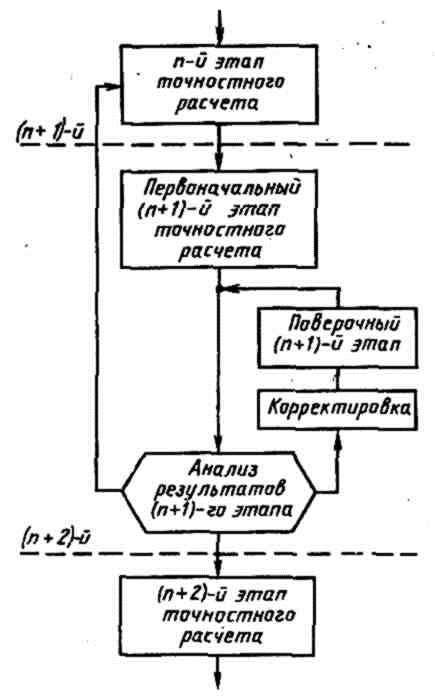
\includegraphics[width=0.4\textwidth]{10algorythm.png}
	\label{pic:10algorythm}
\end{figure}

Если точностный расчет проводится на начальной стадии проектирования, когда не выбрана окончательно структура прибора и невозможно определить его характеристику преобразования и передаточную функцию, приходится достаточно произвольно назначать допуски на погрешности отдельных узлов ОЭП. Эти допуски обычно включают в себя большинство составляющих общей погрешности, поэтому для их расчета можно использовать модель погрешностей (1), приведенную в данной лекции. После проведения точностных расчетов отдельных узлов нужно оценить общую погрешность всего прибора, а при необходимости перераспределить допуски на погрешности между отдельными узлами, между отдельными составляющими в принятой модели погрешностей узлов и прибора в целом, т.е. продолжить итерационный процесс параметрического синтеза~--- определения рациональных параметров прибора, его узлов и деталей, исходя из требований к точности.

\begin{flushleft}
\textbf{Общая методика расчета инструментальных погрешностей}
\end{flushleft}

Методы расчета инструментальных погрешностей очень разнообразны и зависят от особенностей конструкции приборов, принципа их работы и технологии производства. Тем не менее, в специальной литературе содержатся общие рекомендации, определяющие отдельные этапы такого расчета.

Обычно основой расчета инструментальных погрешностей является составление уравнения погрешностей, которое выражает зависимость общей статической погрешности прибора от первичных погрешностей, свойственных отдельным его звеньям или возникающих в этих звеньях под влиянием различных внутренних или внешних факторов. Укажем основные этапы расчета:
\begin{enumerate}
\item анализ процесса измерения и составление структурной схемы прибора;
\item составление рабочей формулы для единичного измерения, т.е. определение функциональной связи между входным и выходным сигналами через параметры отдельных звеньев. Иногда вместо общего коэффициента передачи определяются коэффициенты передачи отдельных звеньев;
\item определение уравнений погрешностей для отдельных звеньев и приведение их к стандартной безразмерной форме;
\item разделение погрешностей на группы по законам их распределения (гауссовский, релеевский, закон Пуассона) и подбор коэффициентов перехода от предельных значений погрешностей к средним квадратическим для каждого закона; выявление систематических погрешностей;
\item составление уравнения погрешностей всего прибора суммированием погрешностей отдельных звеньев с их коэффициентами влияния (весовыми коэффициентами), зависящими от структурной схемы прибора. Это уравнение связывает погрешность выходного сигнала (конечного результата измерения) с частными погрешностями отдельных звеньев и через них с параметрами конструкции и допусками на изготовление отдельных узлов. В соответствии с целью расчета с помощью уравнения погрешностей либо определяется общая инструментальная погрешность прибора, либо это уравнение решается относительно одной из частных погрешностей, что позволяет установить требования к одному из звеньев прибора.
\end{enumerate}

Если известны передаточные коэффициенты отдельных звеньев, то второй и третий этапы составления уравнения погрешностей не вызывают принципиальных затруднений. При этом обычно пользуются разложением в ряд по степеням входного сигнала функций, описывающих связь сигналов на выходе и входе отдельных звеньев. Затем отдельные члены ряда нормируются делением на абсолютную величину выходного сигнала. Более сложным является следующий этап, когда требуется знать или определить законы распределения частных погрешностей.

Один из наиболее сложных моментов точностного расчета~--- выявление источников систематических погрешностей и их учет. Это особенно сложно сделать, если проводятся единичные измерения, хотя и в случае многократных измерений одних и тех же величин борьба с систематическими погрешностями является важнейшей задачей, которую решает конструктор ОЭП.

Уравнение погрешностей прибора позволяет провести анализ соотношения между частными погрешностями, окончательный выбор параметров конструкции и допусков, проверку и уточнение методики измерений для уменьшения влияния систематических погрешностей. Очень часто после разработки конструкции прибора, его изготовления и испытаний необходимо провести дополнительный расчет на максимальное влияние систематических погрешностей, источники которых иногда выявляются лишь в процессе испытаний прибора.

Примеры применения рассмотренной методики подробно описаны в литературе, посвященной расчету и конструированию точных приборов и механизмов, проектированию конкретных типов ОЭП.

\section{Компенсационный метод повышения качества}

Повысить точность (уменьшить погрешность функционирования) оптико-электронного прибора можно технологическим, проектно-конструкторским или компенсационным методами. Компенсационный метод более тесно связан с вопросами проектирования.

Компенсационный метод повышения качества точных приборов широко используется на практике и может дать существенные результаты. Он основан на применении специальных технологических, организационно-технических и конструкторских приемов и устройств (компенсаторов) в целях компенсации влияния погрешностей, ухудшающих показатели качества. Этот метод тесно связан как с технологическим (в случае применения технологических методов компенсации), так и с проектно-конструкторским (в случае конструктивных методов компенсации) методами повышения качества приборов. Специфика оптико-электронных приборов такова, что многие из них выпускаются с компенсаторами тех или иных погрешностей.

Отметим, что при конструировании оптико-электронных функциональных устройств следует предусматривать возможность выполнения их юстировки (регулировки, настройки). Данное правило вызвано спецификой оптико-электронных ФУ, заключающейся в том, что обычно подавляющее большинство из них не может непосредственно после сборки обеспечить необходимые показатели качества (связанные с изображением). Требуется проведение дополнительных мероприятий по устранению и компенсации тех или иных погрешностей путем подвижек, регулировок, деформаций, дополнительной обработки деталей, воздействия на их свойства или результат функционирования~-- т.е. требуется то, что принято называть юстировкой (регулировкой, настройкой).

Обусловлено данное обстоятельство тем, что даже незначительные отклонения характеристик материалов оптических деталей от их номинального значения (в третьем, четвертом и даже пятом знаках после запятой), погрешности изготовления их размеров, формы, расположения приводят к дефектам изображения.

Рассмотрим подробно классификацию \textit{методов компенсации погрешностей} на примере ОЭП.

\begin{flushleft}
\textbf{Технологический метод компенсации}
\end{flushleft}

Заключается в дополнительной обработке деталей прибора, а также в регулировках и юстировках в процессе сборки в целях компенсации отклонений характеристик материалов деталей и погрешностей их изготовления и сборки.

Дополнительная обработка деталей производится, как правило, в процессе их сборки в узлы и называется пригонкой, или доводкой. Доводочные операции осуществляются на металлорежущих станках (установленных на специальном участке сборочного цеха) либо, что чаще, - слесарным способом (шабрением, притиркой, развертыванием, ретушированием). Доводки бывают раздельные, когда каждая деталь подгоняется к эталону (например, с помощью притиров), либо совместные, когда подгоняются друг к другу сопрягаемые детали. Доводка деталей является трудоемким процессом и требует высокой квалификации сборщика-механика.

Регулировки и юстировки осуществляются на завершающем этапе сборки прибора или его узлов путем подвижек деталей либо воздействием на элементы, влияющие на качество ОЭП. Регулировка и юстировка заключаются в выявлении погрешностей, подлежащих компенсации (контроль), устранении (регулировка-юстировка) и фиксации результата.

Заметим, что при применении конструктивных методов компенсации, как правило, не обойтись без регулировок и юстировок таких компенсаторов (т.е. технологической компенсации), что указывает на некоторую условность классификации этих методов. В связи с этим под технологической компенсацией будем понимать только дополнительную обработку деталей.

Данный метод применяется, когда требуется получить высокую надежность компенсации, а также когда другие методы использовать невозможно. В остальных случаях экономически выгоднее применять конструктивный или организационно-технический методы компенсации.

\begin{flushleft}
	\textbf{Организационно-технический метод компенсации}
\end{flushleft}

Заключается, например, в селекции деталей, во введении поправок, пересчете оптической системы прибора на плавки стекол (пересчет для исправления аберраций на фактические значения показателя преломления и средней дисперсии конкретной партии стекла с дальнейшей комплектацией деталей по толщинам и воздушным промежуткам).

Несмотря на некоторые недостатки метода селекции (возможность незавершенного производства, дополнительные затраты на сортировку, нарушение принципа полной взаимозаменяемости), данный метод позволяет компенсировать неблагоприятные сочетания погрешностей изготовления деталей, расширить допуски на точность изготовления их размеров. 

Для компенсации влияния некоторых погрешностей применяются также чисто организационные методы. Например, для компенсации погрешности от мертвого хода рекомендуется производить отсчетные перемещения подвижных систем прибора всегда с одной стороны. Подобным же методом можно уменьшить влияние рефракций воздушных слоев, оказывающих существенное влияние на погрешность функционирования углоизмерительных и других приборов (телескопы, теодолиты, нивелиры, автоколлиматоры), в которых из-за рефракции происходят искривления визирных осей приборов, приводящие к погрешностям измерения, наведения.

К организационно-техническим методам компенсации следует отнести и такие мероприятия, как создание в помещениях, в которых изготавливают и эксплуатируют прецизионные приборы и оборудование, постоянной температуры, давления, влажности, а также устранение сквозняков, вибраций, пыли.

\begin{flushleft}
	\textbf{Конструктивные методы компенсации}
\end{flushleft}

К таким методам относится ввод в конструкцию специальных деталей и устройств для компенсации погрешностей, облегчения оборки, юстировки и выверки прибора.

Конструктивные методы компенсации осуществляются, например, с помощью ступенчатых компенсаторов, регулировочных устройств, механизмов силового замыкания. 

\textit{Ступенчатые компенсаторы} --- это детали, изменением размеров которых добиваются компенсации технологических и других погрешностей приборов. Изменение размеров компенсатора скачкообразное (неплавное), достигается его заменой либо дополнительной технологической обработкой. На рис.~\ref{pic:10kompensator}~а представлен компенсатор \textit{к} (кольцо), заменой либо подрезкой которого добиваются фокусировки объектива.

На рис.~\ref{pic:10kompensator}~б компенсационная прокладка позволяет регулировать зазор оси вращения, на рис.~\ref{pic:10kompensator}~в~-- боковой зазор в зацеплении.

При проектировании этих компенсаторов следует определить их размер и чувствительность, с которой их надо изменять (подбором или обработкой).

\begin{figure}[h!]
	\caption{ Использование простейших конструктивных компенсаторов }
	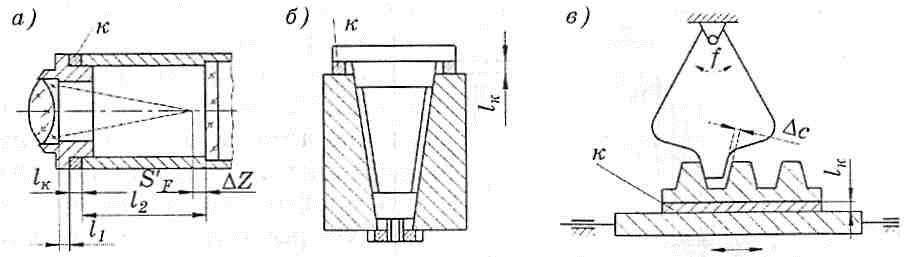
\includegraphics[width=1\textwidth]{10kompensator.png}
	\label{pic:10kompensator}
\end{figure}

Регулировочные устройства в отличие от ступенчатых компенсаторов позволяют плавно изменять размеры и положения деталей и узлов, подвижкой которых обеспечивается требуемое качество.

На рис.~\ref{pic:10regulator} изображено устройство для плавного регулирования зазора в опоре.

\begin{figure}[h!]
	\caption{ Регулировочное устройство }
	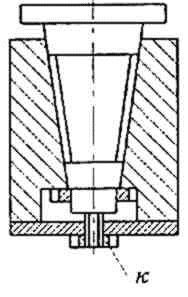
\includegraphics[width=0.2\textwidth]{10regulator.png}
	\label{pic:10regulator}
\end{figure}

Силовое замыкание позволяет компенсировать погрешности изготовления и сборки, а также некоторые эксплуатационные факторы. Пример~--- пружинный подпятник (рис.~\ref{pic:10strongerror}), автоматически выбирающий зазоры, предохраняющий оси от поломки в условиях тряски и вибрации, компенсирующий температурные колебания размеров.

\begin{figure}[h!]
	\caption{ Компенсатор погрешности на основе силового замыкания }
	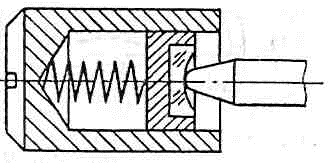
\includegraphics[width=0.45\textwidth]{10strongerror.png}
	\label{pic:10strongerror}
\end{figure}

В зависимости от вида компенсируемых погрешностей и <<места>> регулировки (изменения параметров) компенсаторы можно подразделить на регулировочно-юстировочные, функциональные, настроечно-выверочные.

\textit{Регулировочно-юстировочные компенсаторы} предназначены для компенсации погрешностей отдельных деталей и размерных цепей. Их параметры изменяются при выполнении регулировок и юстировок прибора. Типичными представителями компенсаторов этого типа являются кольца для фокусировки объективов, прокладки для регулировки зазоров в кинематических парах, доводка направляющих, регулировочные устройства для центрировки объективов и зеркально-призменных систем.

\textit{Функциональные компенсаторы} предназначены для компенсации переменных погрешностей функциональных преобразователей прибора. Их параметры изменяются при эксплуатации ОЭП. Примерами такого типа компенсаторов могут служить коррекционные устройства, температурные компенсаторы, устройства стабилизации линии визирования, оптические адаптивные компенсаторы, алгоритмическая компенсация с помощью микроЭВМ.

\textit{Настроечно-выверочные компенсаторы} предназначены для компенсации погрешностей ориентации прибора, износа, расстройки. Параметры этих компенсаторов изменяются в процессе настройки и выверки прибора. К компенсаторам данного типа относятся, например, устройства для выверки оптических дальномеров по высоте и дальности, устройства выверки теодолита в полевых условиях для устранения наклона вертикальной, горизонтальной осей вращения и коллимационной ошибки, регулировочные устройства, предназначенные для компенсации износа направляющих, компенсации изменения моментов и сил на рукоятках управления, устройства калибровки преобразователей автоматизированных ОЭП.

\section{Структурные схемы компенсации погрешностей}

Представим компенсацию погрешностей ОЭП в виде следующей структурной схемы (рис.~\ref{pic:10schemeerror}), где $ x,\, y $ -- информативные параметры входного и выходного сигналов; $ q $ -- конструктивные параметры прибора; $ q' $ -- влияющие факторы (рефракция воздушных слоев, температура, вибрации, номиналы источников электропитания); $ f $ -- функция, связывающая $ x $ и $ y $; $ x_0,\, y_0,\, q_0,\, q,\, f_0 $~-- расчетные (номинальные) значения перечисленных параметров; $ \Delta z_k $ -- управляющий сигнал на компенсатор; $ \Delta x_k $ -- коррекция, вырабатываемая компенсатором, поступающая на вход прибора; $ \Delta y_k $~-- коррекция компенсатора, подаваемая на выход прибора (т.е. коррекция информативного параметра выходного сигнала); $ \Delta q_k $ -- коррекция компенсатора, изменяющая параметры прибора. 

Допущения относительно объекта измерения, инструментальные погрешности, погрешности регистрации и погрешности, возникающие из-за изменения влияющих факторов приводят к ухудшению качества прибора ($ \Delta y = y - y_0 $).

\begin{figure}[h!]
	\caption{ Структурная схема компенсации погрешностей:
%	1 -- объект (наблюдения, измерения, управления), 2 -- оптико-электронный прибор, 3 -- измерительное, образцовое (эталонное), вычислительное устройство,	4 -- система сравнения погрешности(ей) и показателей качества ОЭП с ее (их) допустимыми значениями,\\ 5 -- компенсатор}
	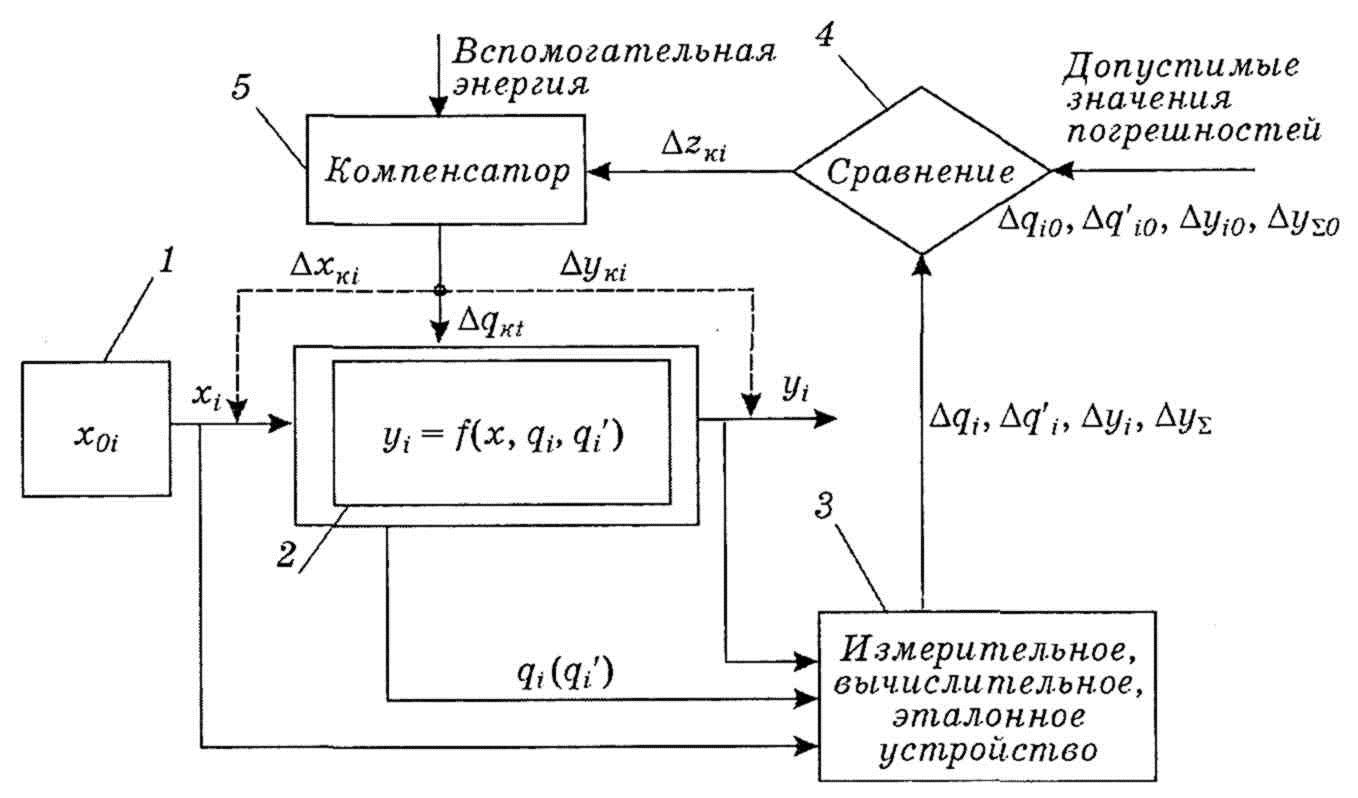
\includegraphics[width=1\textwidth]{10schemeerror.png}
	\label{pic:10schemeerror}
\end{figure}

В общем случае компенсатор в зависимости от погрешностей прибора, входного или выходного информативного параметра, влияющих факторов вырабатывает (при необходимости с использованием вспомогательной энергии) коррекционное воздействие, которое изменяет конструктивные параметры прибора либо его входной или выходной сигнал, так что устраняется (компенсируется) либо результат действия погрешности на тот или иной показатель качества, либо сама погрешность. Для выработки коррекционного воздействия необходим управлявший сигнал на компенсатор $ \Delta z_k $, который создается с помощью системы сравнения.

Управляющий сигнал на компенсатор представляет собой в общем виде электрическое, механическое и подобное воздействие на параметры компенсатора.
В зависимости от способов получения управляющего сигнала структурные схемы компенсации погрешностей ОЭП могут быть построены по следующим схемам: схеме вспомогательных измерений, схеме образцовых сигналов, схеме обратного преобразования. Наибольшее распространение в ОЭП получили первые две схемы коррекции, их комбинация, а также схема цифровой (алгоритмической) коррекции. (Всего 4 схемы, при юстировке -- 2 схемы).

\begin{flushleft}
	\textbf{Компенсация по схеме вспомогательных измерений}
\end{flushleft}

Заключается в том, что погрешности параметров и изменения влияющих факторов либо их частичные влияния измеряются с помощью вспомогательных измерительных устройств (рис.~\ref{pic:10compensation}). Их роль выполняют обычно контрольно-измерительные приборы и средства: измерительные микроскопы, автоколлиматоры, приборы измерения линейных величин (индикаторы, оптиметры, интерферометры и т.п.), фазометры, осциллографы, датчики температуры и давления, лекальные линейки, пробные стекла.

Измеренные значения погрешностей поступают затем в систему (устройство) сравнения, функцию которого выполняет, например, при автоматизированной коррекции процессор, а при неавтоматизированной --- оператор. 

В системе сравнения заложена зависимость частичных показателей качества ($ \Delta y_{\Delta q} $, $ \Delta y_{\Delta q'} $) от первичных погрешностей и факторов ($ \Delta y_{\Delta q, \Delta q'} = f(x,\,y,\, q_i, \, \Delta q_i,\, \Delta q_{i'}) $) а также допустимые значения первичных погрешностей и факторов ($ \Delta q_{i0},\, \Delta q'_{i0} $) и их влияний ($ \Delta y_{\Delta q_{i0}},\, \Delta y_{\Delta q'_{i0}} $) виде численных значений, таблиц или графиков.

На основании сравнения измеренных первичных погрешностей и факторов с их допустимыми значениями (либо действительного и допустимого влияния погрешностей) система сравнения вырабатывает при $ \Delta q_i > \Delta q_{i0} $, $ \Delta y_{\Delta q_i} > \Delta y_{\Delta q_{i0}} $ управляющий сигнал на компенсатор(ы) $ \Delta z_k $. Управляющий сигнал изменяет параметры компенсатора, в результате чего он воздействует на параметры прибора $ \Delta q_k $ либо на информативные параметры $ x $, $ y(\Delta x_k,\, \Delta y_k ) $ в целях устранения самой погрешности или ее влияния на качество.

\begin{figure}[h!]
	\caption{ Компенсация по схеме вспомогательных измерений }
	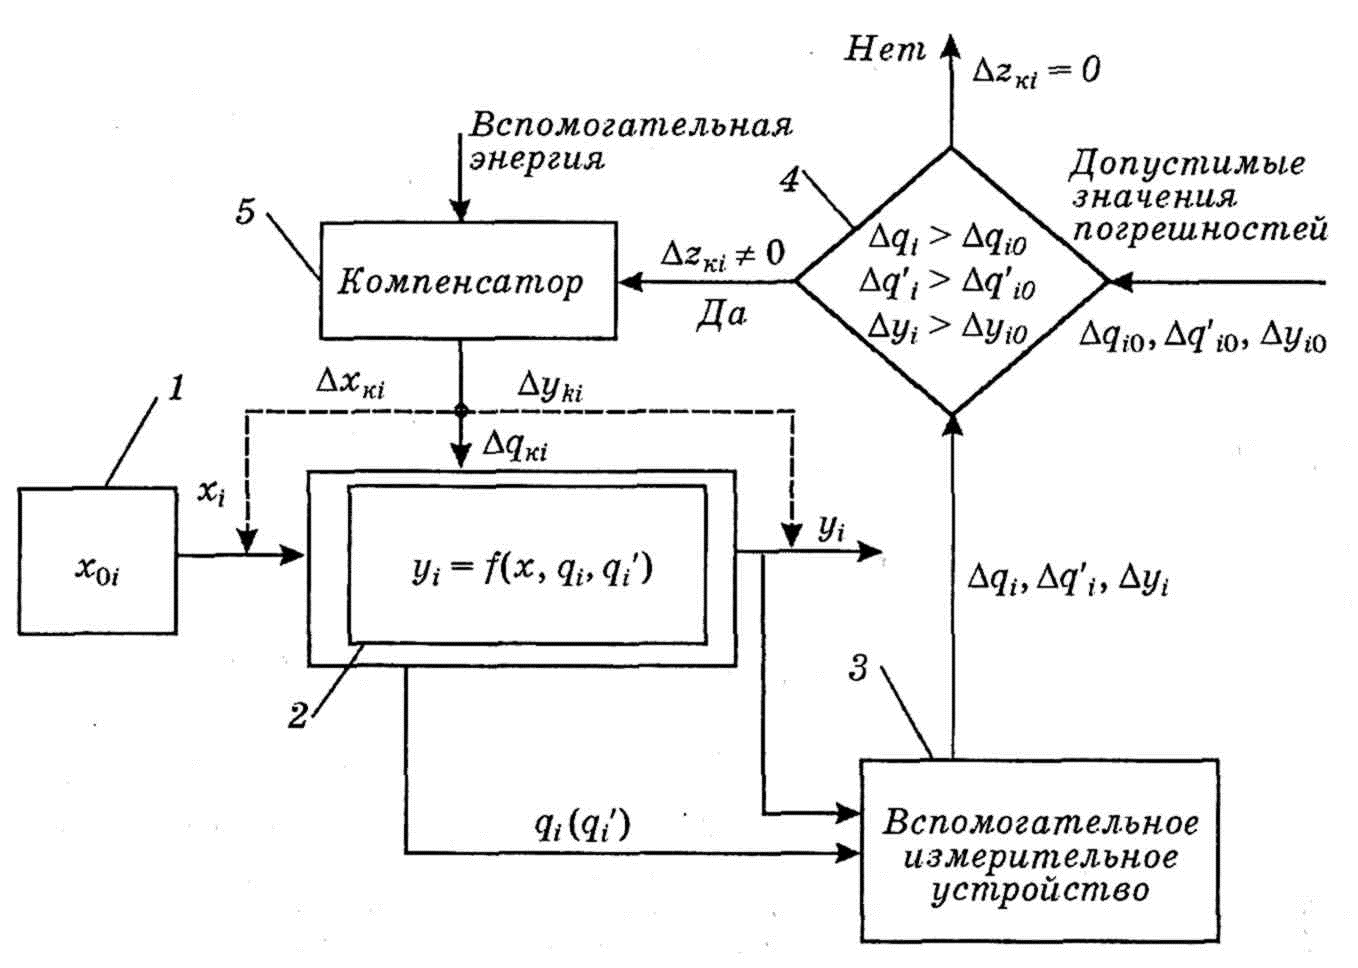
\includegraphics[width=0.9\textwidth]{10compensation.png}
	\label{pic:10compensation}
\end{figure}

\begin{flushleft}
	\textbf{Компенсация по схеме образцовых сигналов}
\end{flushleft}

Основана на том, что на вход прибора подается образцовый сигнал $ x_0 $ либо в состав системы коррекции входит образцовый (эталонный) преобразователь (рис.~\ref{pic:10etalon}). Образцовый сигнал позволяет получить номинальное значение $ y_0 $ информативного параметра выходного сигнала путем расчета по номинальной функции прибора, а образцовый прямой преобразователь (эталонный прибор) --- номинальным (эталонным) преобразованием сигнала.

\begin{figure}[h!]
	\caption{ Компенсация по схеме образцовых сигналов }
	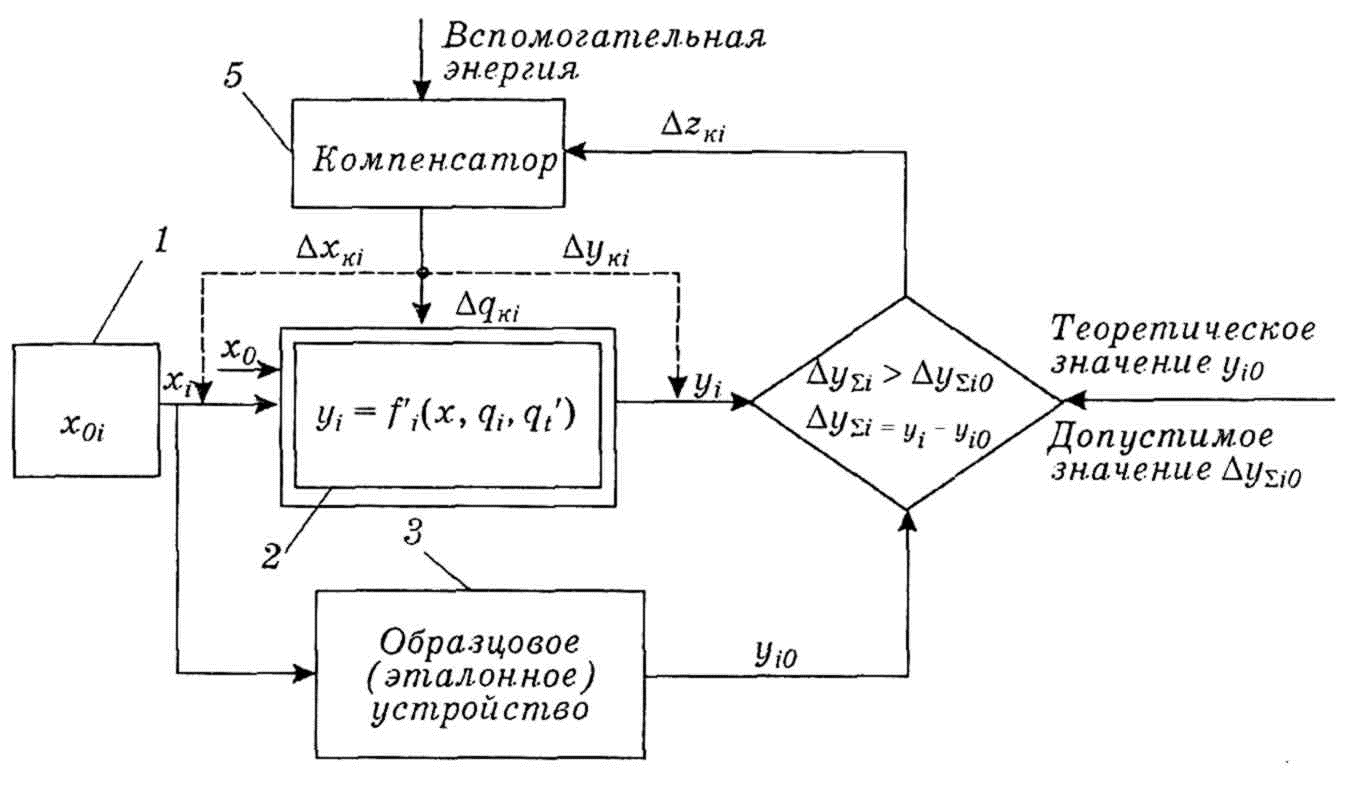
\includegraphics[width=1\textwidth]{10etalon.png}
	\label{pic:10etalon}
\end{figure}

Номинальное значение $ y_0 $ поступает в систему сравнения, где вычисляется разность значения $ y_0 $ и действительного его значения $ y $, поступившего с выхода прибора: $ \Delta y = y - y_0 $.

Система сравнения на основании сравнения $ \Delta y $ с его допустимым значением $ \Delta y_0 $ вырабатывает при $ \Delta y > \Delta y_0 $ управляющий сигнал на компенсатор.

В качестве образцового сигнала используют: волновой фронт эталонного источника светового излучения; эталоны угловых и линейных величин (шкалы, концевые меры, призмы, коллиматоры); углы и расстояния между предметами, звездами, длины волн спектральных линий.

Образцовыми преобразователями могут быть эталонные приборы, объективы, оптические микрометры, датчики, источники и приемники оптического излучения.

По схеме образцовых сигналов обычно производятся компенсация погрешностей при окончательной юстировке прибора или его функциональных узлов, калибровка измерительных приборов по эталонным мерам, объектам и приборам. 

\begin{flushleft}
	\textbf{Компенсация по схеме цифровой (алгоритмической) коррекции}
\end{flushleft}

Заключается в том, что входящее в систему коррекции вычислительное устройство (ВУ) 3 -- микропроцессор, микроконтроллер, персональный компьютер -- вводит в результат функционирования ОЭП поправки для компенсации влияния погрешностей (рис.~\ref{pic:10digital}). Эти поправки вычисляются по определенному алгоритму для текущего значения информативного параметра выходного сигнала. Алгоритм закладывается в память ВУ на основе теоретического анализа влияния тех или иных погрешностей и факторов либо результатов их измерений.

\begin{figure}[h!]
	\caption{ Компенсация по схеме цифровой (алгоритмической) коррекции }
	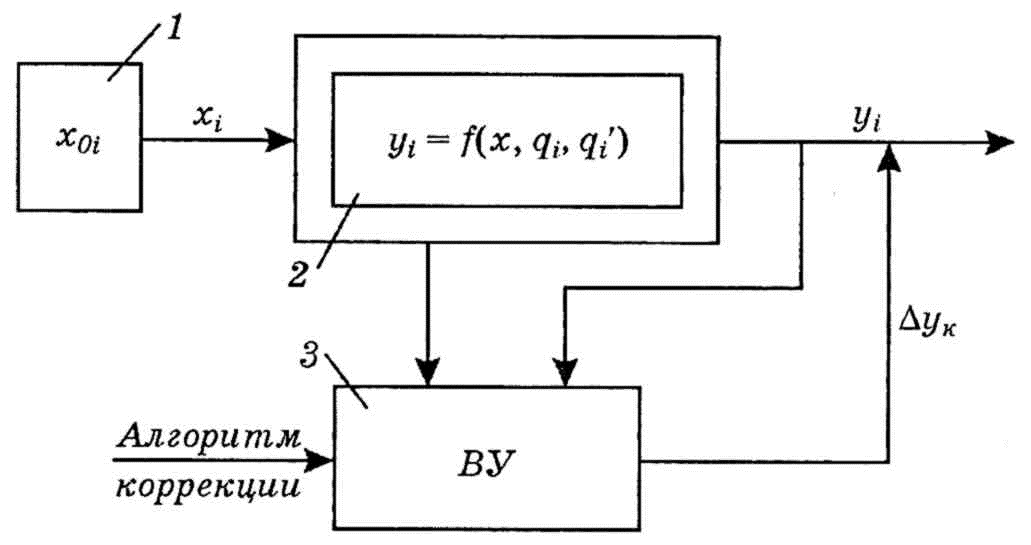
\includegraphics[width=0.6\textwidth]{10digital.png}
	\label{pic:10digital}
\end{figure}

По такой схеме компенсируют, например, влияние теоретических погрешностей, систематических технологических и эксплуатационных погрешностей, а также случайных погрешностей путем усреднения результатов при повторных циклах функционирования по одному и тому же входному сигналу. 

Компенсация по схеме цифровой (алгоритмической) коррекции обладает следующими особенностями:
\begin{itemize}
\item возможна коррекция как систематических, так и случайных погрешностей;
\item необходимо определение корректирующей функции и алгоритма коррекции погрешностей;
\item точность коррекции в существенной степени зависит от точности корректирующей функции, оптимальности алгоритма и точности его привязки к информативному параметру выходного сигнала.
\end{itemize}

Довольно часто компенсация погрешностей ОЭП построена по смешанной схеме: при поузловой сборке применяется схема вспомогательных измерений, окончательная корректировка осуществляется по схеме образцовых сигналов, а компенсацию теоретических и эксплуатационных погрешностей выполняют по схеме цифровой (алгоритмической) коррекции.

В заключение следует отметить некоторые тенденции и факторы, влияющие на точность приборов и ее расчет.
\begin{enumerate}
\item Наблюдается тенденция упрощения конструкций прецизионных приборов благодаря:
\begin{itemize}
\item использованию новых материалов, обладающих лучшими и стабильными характеристиками;
\item появлению более высококачественных и многофункциональных элементов и устройств, например, подшипников, источников и приемников излучения, датчиков, преобразователей, двигателей и т. д.;
\item замене относительно сложных оптико-механических и электромеханических функциональных устройств прибора конструктивно более простыми электронными и микропроцессорными функциональными устройствами.
\end{itemize}
Данное обстоятельство уменьшает количество источников и значение первичных погрешностей в современных приборах.
\item Широкое применение базовой и блочно-модульной унификации конструкций при проектировании современных приборов позволяет не только повысить ряд показателей его качества, сократить сроки проектирования, обеспечить экономическую эффективность и т.п., но и существенно упростить расчет суммарной погрешности, так как значения погрешностей (иногда также их подробные характеристики для конкретных экземпляров) унифицированных элементов и устройств даны в их технических паспортах или описаниях.
\item Использование в составе современных оптических и других точных приборов микропроцессорной техники и персональных компьютеров позволяет помимо автоматизации процесса  их функционирования осуществлять цифровую (алгоритмическую) коррекцию частичных или суммарной погрешностей, что, как известно, существенно повышает их точностные характеристики.
\item Использование в процессе проектирования компьютерной техники и систем (САПР), специальных программ для точностного анализа и синтеза позволяет оптимизировать параметры и характеристики элементов и устройств прибора с позиции точности, ускорить и облегчить процесс вычислений.
В связи с вышеизложенным можно утверждать, что в настоящее время точностной анализ и синтез приборов превращается из искусства, которым хорошо владел относительно узкий круг специалистов, в обычный этап проектирования, доступный каждому конструктору.
\end{enumerate}
